\documentclass[conference]{IEEEtran}

\IEEEoverridecommandlockouts
\usepackage{cite}
\usepackage{amsmath,amssymb,amsfonts}
\usepackage{algorithmic}
\usepackage{graphicx}
\usepackage{textcomp}
\usepackage{xcolor}
\usepackage{times}
\usepackage{caption}
\usepackage{subcaption}
\usepackage{url}
\usepackage{placeins}

% Let floats fill more of a page so they stay near the text that cites them
\renewcommand{\topfraction}{0.9}
\renewcommand{\bottomfraction}{0.8}
\renewcommand{\textfraction}{0.1}
\renewcommand{\floatpagefraction}{0.8}
\renewcommand{\dbltopfraction}{0.9}
\renewcommand{\dblfloatpagefraction}{0.8}
\setcounter{topnumber}{3}
\setcounter{totalnumber}{5}
\def\BibTeX{{\rm B\kern-.05em{\sc i\kern-.025em b}\kern-.08em
    T\kern-.1667em\lower.7ex\hbox{E}\kern-.125emX}}

\begin{document}

\title{Does Income Volatility Matter for Retirement Asset Allocation? A PLFS-Calibrated Simulation Study of India's National Pension System}

\author{
\IEEEauthorblockN{[Author 1 Name]}
\IEEEauthorblockA{\textit{Department of [Department]} \\
\textit{[Institute]}\\
[City, State, Country] \\
[email]}
\and
\IEEEauthorblockN{[Author 2 Name]}
\IEEEauthorblockA{\textit{Department of [Department]} \\
\textit{[Institute]}\\
[City, State, Country] \\
[email]}
\and
\IEEEauthorblockN{[Guide / Author 3 Name]}
\IEEEauthorblockA{\textit{Department of [Department]} \\
\textit{[Institute]}\\
[City, State, Country] \\
[email]}
}

\maketitle

\begin{abstract}
India's National Pension System (NPS) places subscribers who make no active choice into an age-based ``Auto Choice'' life-cycle fund whose allocation depends on age alone. Informal workers, who form roughly 78\% of the workforce, contribute irregularly, which suggests that an allocation conditioned on income volatility might serve them better. Because subscriber-level NPS data are not public, we build a reproducible simulation framework that combines real NPS NAV history (SBI Pension Funds, Tier~I, 2009--2026, block bootstrap) with a synthetic subscriber population calibrated to the Periodic Labour Force Survey (PLFS) 2023--24. We evaluate glide paths on terminal-corpus attainment, intra-horizon shortfall, money-weighted return and a disruption-triggered withdrawal channel, and test the volatility-conditioning hypothesis through a progressive sequence of objectives, a risk-budget (Pareto-frontier) formulation, an equity-premium stress test and a 54-cell robustness study with paired bootstrap confidence intervals. Income volatility strongly affects accumulation: informal cohorts skip about 10\% of contribution months versus 0.07\% for salaried workers, and, when every disruption month triggers a withdrawal, median corpus falls by 79--92\% for the informal tiers. It does not, however, change the optimal allocation: the optimal glide path is governed by the equity premium over government securities, switching from maximum to minimum equity at a premium of roughly 0--1\% per year, and tier-conditioned policies are statistically indistinguishable from tier-blind ones in all 54 robustness cells (largest gain 0.004). We conclude that the leverage on informal-worker outcomes lies in contribution regularity and liquidity design rather than in volatility-conditioned glide paths, and we release a risk-budget recommender built on the same engine.
\end{abstract}

\begin{IEEEkeywords}
National Pension System, glide path, asset allocation, informal sector, Monte Carlo simulation, sequence-of-returns risk, risk budget
\end{IEEEkeywords}

%--------------------------------------------------------------------------
\section{Introduction}
India's National Pension System (NPS) assigns subscribers who do not actively choose an investment pattern to the ``Auto Choice'' life-cycle fund (LC50 by default; LC75 and LC25 optional), whose equity, corporate-debt and government-securities weights follow a fixed schedule in age alone \cite{pfrda}. Such schedules implicitly assume a steadily contributing, salaried saver. Self-employed and casual workers, however, constitute about 78\% of the workforce in the Periodic Labour Force Survey (PLFS) 2023--24 \cite{plfs} and earn and contribute irregularly. The natural hypothesis (H1) is that an allocation conditioned on income volatility would outperform an age-only schedule for this population.

Testing H1 directly is difficult because subscriber-level NPS records are not publicly available. We therefore construct a simulation environment from two sources that \emph{are} public: real NPS scheme NAV history, which supplies realistic return dynamics, and PLFS aggregate statistics, which calibrate a synthetic population of subscribers with heterogeneous income volatility. Every quantity that is not measured from these sources is recorded in an explicit assumption register (Table~\ref{tab:assump}). Fig.~\ref{fig:pipeline} gives an overview of the framework.

\begin{figure*}[!t]
\centering
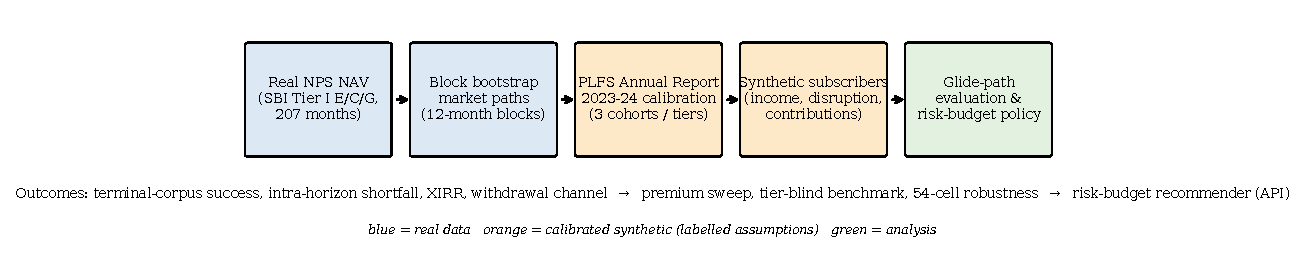
\includegraphics[width=\textwidth]{figures/fig1_pipeline.pdf}
\caption{Overview of the framework. Real NAV history drives bootstrapped market paths; PLFS statistics calibrate synthetic subscribers; glide paths are evaluated on terminal, path-dependent and liquidity metrics and then analysed through risk-budget, premium-stress and robustness studies.}
\label{fig:pipeline}
\end{figure*}

Rather than test H1 with a single objective, we examine it through a progressive sequence of increasingly demanding formulations: terminal-wealth objectives, a path-dependent shortfall objective, a combined growth--shortfall objective, a liquidity (forced-withdrawal) channel, a risk-budget Pareto formulation, an equity-premium stress test and a systematic perturbation study. This sequence yields a consistent and, we argue, informative answer: income volatility is a first-order determinant of \emph{how much} informal workers accumulate, but not of \emph{how} their savings should be allocated.

The contributions of this paper are:
\begin{enumerate}
\item A reproducible hybrid framework (real NAV + PLFS-calibrated synthetic subscribers) with all non-measured assumptions labelled and perturbed.
\item Path-dependent risk measures---intra-horizon shortfall and money-weighted return---and a liquidity channel tied to calibrated disruption months.
\item A risk-budget formulation (maximize target attainment subject to a cap on shortfall probability) with Pareto frontiers by volatility tier.
\item An equity-premium break-even analysis showing that the optimal allocation is set by the market premium and decouples from income volatility.
\item A 54-cell robustness study in which no confidence interval for the benefit of volatility conditioning excludes zero, together with an open risk-budget recommender.
\end{enumerate}

%--------------------------------------------------------------------------
\section{Related Work}
\textbf{Life-cycle portfolio choice.} The classical results of Merton and Samuelson \cite{merton,samuelson} established that optimal risky-asset exposure depends on risk preferences and return dynamics. Subsequent work added labor income: human capital acts as an implicit bond-like asset, so that risky holdings should be higher early in life \cite{bms,viceira}, and calibrated life-cycle models reproduce hump-shaped or declining equity shares \cite{cgm,gm,cv}. In these frameworks income risk influences allocation through its correlation with asset returns and through precautionary motives. Our setting differs in that the saver's \emph{contributions}, not a consumption--saving trade-off, are volatile, and the policy class is a fixed glide path as in practice.

\textbf{Glide paths and sequence risk.} Target-date and life-cycle funds de-risk with age, partly to limit sequence-of-returns risk near the decumulation date; the historical sequencing of returns is known to matter for outcomes when cash flows are not constant \cite{bengen}. We contribute path-dependent measures (intra-horizon shortfall, money-weighted return) designed to expose sequence risk arising from irregular \emph{inflows}.

\textbf{Resampling methods.} We generate market scenarios by a moving-block bootstrap of real monthly returns \cite{efron,kunsch,politis}, which preserves cross-asset correlation and regime structure.

\textbf{Indian context.} PFRDA publishes the Auto Choice allocation tables and annual statistics \cite{pfrda}, and PLFS reports employment status, earnings and unemployment by worker type \cite{plfs}. To our knowledge the question of whether volatility-conditioned allocation benefits informal NPS subscribers has not been examined with a calibrated simulation of this kind; this paper does so and reports a quantitative answer.

%--------------------------------------------------------------------------
\section{Data and Calibration}
\subsection{Market data}
We use daily NAV for the SBI Pension Funds Tier~I equity (E), corporate-debt (C) and government-securities (G) schemes from 5~May 2009 to 10~August 2026, obtained from an open NAV service \cite{npsnav}. Daily log returns are aggregated to monthly returns. The fund's first calendar month is a flat-NAV launch period and is excluded, leaving $207$ monthly observations (June 2009--August 2026). Over this pool equity returned $11.5\%$ per year on average against $8.5\%$ for G-secs, an equity premium of $2.9\%$ per year---the single most important feature of the data for what follows.

\subsection{PLFS calibration and volatility tiers}
Three cohorts are calibrated from national tables of PLFS 2023--24 \cite{plfs} (employment-type shares; quarterly earnings by employment type, location and gender; unemployment rate). For each cohort we compute a measured between-cell coefficient of variation (CV) of earnings from 16 published cells (4 quarters $\times$ rural/urban $\times$ gender). Because published tables do not give individual-level dispersion, an assumed multiplier maps the measured CV to a target individual CV; the resulting ordering defines three volatility tiers (Table~\ref{tab:calib}).

\begin{table}[!htbp]
\centering
\caption{PLFS-calibrated cohorts and volatility tiers}
\label{tab:calib}
\begin{tabular}{lccccc}
\hline
Cohort & Share & Mean inc. & Meas. & Mult. & Target \\
 & (\%) & (Rs/mo) & CV & (assumed) & CV; tier \\
\hline
Regular salaried & 21.7 & 20,702 & 0.267 & 1.3 & 0.35; low \\
Casual labour & 19.8 & 10,032 & 0.230 & 2.5 & 0.58; medium \\
Self-employed & 58.4 & 13,279 & 0.559 & 2.0 & 1.12; high \\
\hline
\end{tabular}
\end{table}

The self-employed show by far the largest measured dispersion (rural-female and urban-male self-employment earnings differ more than fourfold), an ordering that emerges from the data before any assumption is applied.

%--------------------------------------------------------------------------
\section{Simulation Framework}
\subsection{Synthetic subscribers}
We simulate $N=2{,}000$ subscribers, assigned to cohorts with PLFS shares, over $T=432$ months (ages 25--60, the standard NPS retirement age). For subscriber $i$, monthly income is
\begin{equation}
y_{i,t}=b_i\,g^{t}\,s_{i,t}\,\exp(\eta_{i,t})\,\delta_{i,t},
\end{equation}
where $b_i$ is a lognormal baseline fitted by method of moments to the cohort mean and the cross-sectional share of the target CV, $g$ a growth factor, $s_{i,t}$ a seasonal factor (agriculture and construction only), $\eta_{i,t}$ an AR(1) shock whose stationary variance matches the temporal share of the CV, and $\delta_{i,t}\in(0,1]$ a disruption factor applied in Bernoulli disruption months whose probability is anchored to the PLFS unemployment rate (4.9\%) and scaled by cohort. Contributions are
\begin{equation}
c_{i,t}=\pi_k\,\max(0,\;y_{i,t}-F),
\end{equation}
with cohort propensity $\pi_k$ and subsistence floor $F$, and are further skipped with a cohort-specific probability in disruption months. Contribution irregularity is therefore an \emph{emergent} property of calibrated volatility rather than an imposed one.

\subsection{Glide paths and baselines}
PFRDA's LC25, LC50 and LC75 age tables are transcribed and used as baselines. The candidate policy class is a three-parameter glide path: starting equity $e_0$, ending equity $e_1$ and inflection age $a$, with equity held at $e_0$ until $a$, declining linearly to age 55 and held at $e_1$ thereafter; the non-equity remainder is split 35/65 between corporate debt and G-secs.

\subsection{Outcome measures}
For market path $m$ (monthly portfolio return $\rho_{m,t}$) the corpus evolves as
\begin{equation}
C_{i,t}=C_{i,t-1}(1+\rho_{m,t})+c_{i,t}-W_{i,t},
\end{equation}
where $W_{i,t}=\phi\,C_{i,t}$ with probability $p$ in a disruption month and $0$ otherwise (the liquidity channel; $\phi=10\%$). We report:
\begin{itemize}
\item \textbf{Success} $S=\Pr(C_{i,T}\ge \bar C)$, with $\bar C$ the tier's median terminal corpus under LC50 in the same scenario.
\item \textbf{Intra-horizon shortfall} $H=\Pr\big(\exists t:\;(C_{i,t}+\sum_{u\le t}W_{i,u})/\sum_{u\le t}c_{i,u}<0.9\big)$, evaluated once cumulative contributions exceed Rs~1{,}000.
\item \textbf{Money-weighted return} (XIRR) $r$ solving $\sum_t c_{i,t}(1+r)^{-t}=C_{i,T}(1+r)^{-(T-1)}$, computed with a vectorized Newton solver.
\end{itemize}
Shortfall is deliberately path-dependent: unlike terminal wealth it is sensitive to when returns occur relative to contributions.

\subsection{Risk-budget formulation}
For a risk budget $\varepsilon$ the policy solves
\begin{equation}
\max_{\theta}\; S(\theta)\quad\text{s.t.}\quad H(\theta)\le\varepsilon,
\end{equation}
over the candidate grid $\theta=(e_0,e_1,a)$. Each candidate is simulated once per tier with common random numbers, so Pareto frontiers, $\varepsilon$-constrained optima and scalarized optima $S-\lambda H$ are all selections from one table. A \emph{tier-blind} benchmark maximizes the subscriber-weighted average objective over all tiers. Candidates are selected on one random seed (100 market trials) and evaluated on a different seed (200 trials).

\subsection{Verification}
The XIRR solver was validated against four closed-form cases (single payoff, exact recovery of a known compounding rate, a break-even case and a multi-trial vectorization check); cells where Newton's method does not converge ($1$--$2.3\%$) are reported as missing and excluded from averages rather than clipped. The market engine was audited, leading to the exclusion of the flat-NAV launch month. All simulations use explicit seeds.

\begin{table}[!htbp]
\centering
\caption{Assumption register: quantities not measured from data}
\label{tab:assump}
\small
\begin{tabular}{ll}
\hline
Parameter & Value (sal./casual/self-emp.) \\
\hline
Individual-dispersion multiplier & 1.3 / 2.5 / 2.0 \\
Cross-sectional share of CV & 0.5 \\
AR(1) persistence $\rho$ & 0.10 / 0.55 / 0.45 \\
Annual income growth & 6\% / 4\% / 5\% \\
Disruption prob. (multiple of 4.9\%) & 0.3 / 3.0 / 1.5 \\
Contribution propensity $\pi_k$ & 0.20 / 0.08 / 0.10 \\
Subsistence floor $F$ & Rs 5,000 \\
Casual daily$\to$monthly wage & 24 days \\
Withdrawal fraction $\phi$ & 10\% of corpus \\
Shortfall threshold; min. contrib. & 0.9; Rs 1,000 \\
Corporate share of non-equity & 35\% \\
Bootstrap block length & 12 months \\
\hline
\end{tabular}
\end{table}

%--------------------------------------------------------------------------
\section{Experimental Design: A Progressive Test of H1}
We test H1 through five stages, each designed to remove a possible reason why conditioning on volatility might have failed to show a benefit in the previous one.
\begin{enumerate}
\item[\textbf{E1}] \emph{Terminal wealth.} Does the optimal glide path for maximizing target attainment differ by tier?
\item[\textbf{E2}] \emph{Sequence risk.} Does a path-dependent objective (minimizing shortfall) separate the tiers?
\item[\textbf{E3}] \emph{Growth--risk trade-off.} Because E1 and E2 are one-sided, we combine them (scalarized $S-\lambda H$) and, to avoid dependence on $\lambda$, analyse the full Pareto frontier and risk-budget policy.
\item[\textbf{E4}] \emph{Liquidity.} We add disruption-triggered withdrawals, the mechanism through which income volatility could most plausibly interact with market timing.
\item[\textbf{E5}] \emph{Is it the market window?} We subtract a constant premium haircut from every bootstrapped equity month and repeat E1 (with and without withdrawals), then perturb every income assumption in Table~\ref{tab:assump} that could plausibly create or mask a tier effect (disruption rate, propensity, dispersion, subsistence floor).
\end{enumerate}

%--------------------------------------------------------------------------
\FloatBarrier
\section{Results}
\subsection{R1: Volatility strongly affects accumulation}
Informal cohorts skip roughly one contribution month in ten: $10.20\%$ of months for the self-employed and $10.05\%$ for casual labour, against $0.07\%$ for regular salaried workers, a gap of about $150\times$ (Fig.~\ref{fig:acc} (top)). Median terminal corpus under LC50 is Rs~24.4M, 2.6M and 6.0M for the low, medium and high tiers (Fig.~\ref{fig:acc} (bottom)); the medium tier ends below the high tier because tiers rank income \emph{volatility}, while the self-employed earn and contribute more in absolute terms. LC75 improves on LC50 in every tier, a first indication of how favourable the sample period was to equity.

\begin{figure}[!htbp]
\centering
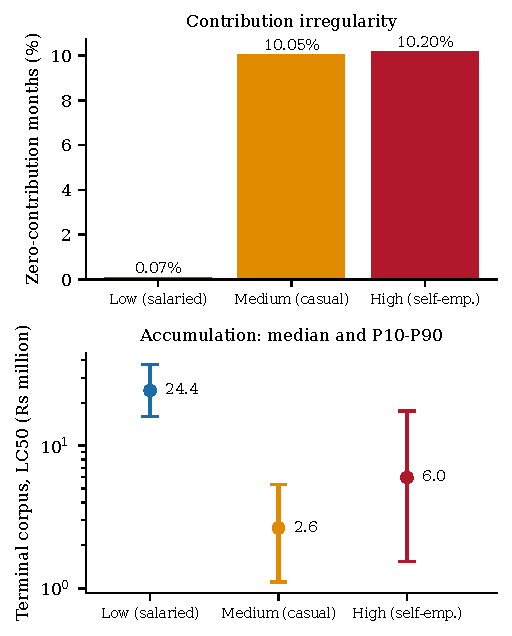
\includegraphics[width=0.95\columnwidth]{figures/fig2_accumulation.pdf}
\caption{(Top) Share of months with zero contribution by tier. (Bottom) Terminal corpus under LC50 (median and P10--P90, log scale; $n=200$ market paths).}
\label{fig:acc}
\end{figure}

\subsection{R2: Pure objectives select the same corner in every tier (E1--E3)}
Maximizing target attainment selects $75\%$ starting equity in all three tiers; minimizing shortfall selects $15\%$ in all three (Fig.~\ref{fig:ladder}). The two objectives therefore yield mirror-image corner solutions, neither of which expresses the trade-off a saver faces. An initial scalarized objective ($\lambda=1$) evaluated on a coarse five-point equity grid returned a split across tiers ($60/60/45\%$); on a refined grid and on the full candidate table the scalarized optimum is $45\%$ in every tier, i.e.\ the split reflected where the scalarized optimum fell between coarse grid points rather than a tier effect. We therefore use the grid-independent frontier analysis below as the primary evidence.

\begin{figure}[!htbp]
\centering
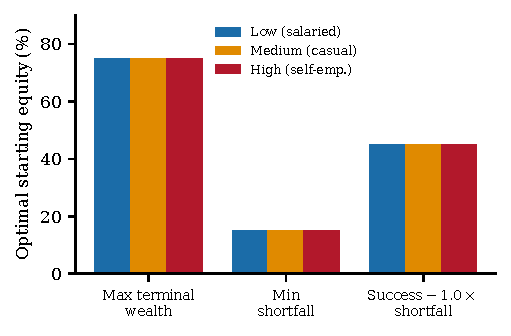
\includegraphics[width=0.9\columnwidth]{figures/fig3_objective_ladder.pdf}
\caption{Optimal starting equity by objective and tier. Each objective selects the same allocation in all tiers.}
\label{fig:ladder}
\end{figure}

\subsection{R3: Risk-budget frontiers are nearly tier-invariant}
The mapping from allocation to shortfall risk along the Pareto frontier is almost identical across tiers (Fig.~\ref{fig:frontier} (top)); success levels differ (Fig.~\ref{fig:frontier} (bottom)) only because each tier is judged against its own target. At the maximum-equity candidate the shortfall probability is $0.172$, $0.175$ and $0.182$ for the low, medium and high tiers. Table~\ref{tab:eps} reports the risk-budget policy. For budgets $\varepsilon\in\{0.02,0.10,0.15,0.20\}$ the tier-conditioned and tier-blind policies are identical. At the tightest budgets ($\varepsilon=0.01,0.05$) they differ by one 10-point grid step, because the small between-tier shortfall differences place a grid candidate on opposite sides of the budget: at $\varepsilon=0.01$ the low and medium tiers can hold 45\% equity (success gains $+0.031$ and $+0.020$), while at $\varepsilon=0.05$ the tier-blind policy's 55\% equity for the low tier exceeds the budget out-of-sample (0.059). Thus volatility enters the risk-budget problem only through a small shift in feasibility at tight budgets, not through a different allocation logic.

\begin{figure}[!htbp]
\centering
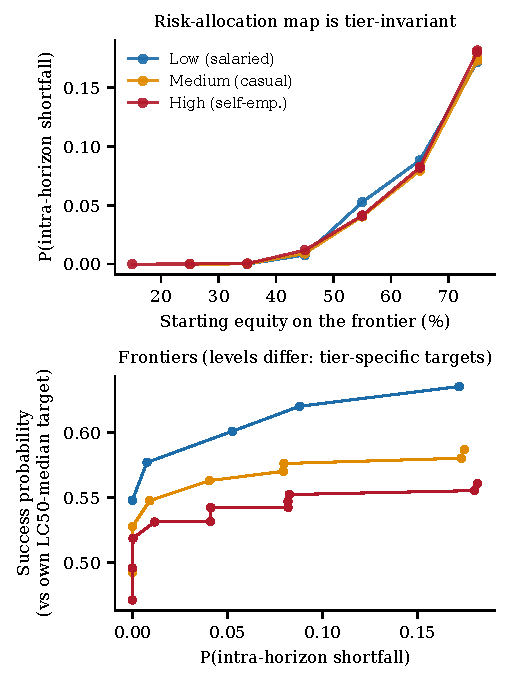
\includegraphics[width=0.95\columnwidth]{figures/fig4_frontiers.pdf}
\caption{Pareto frontiers by tier. (Top) Intra-horizon shortfall probability versus starting equity on the frontier: the risk-allocation map is almost identical across tiers. (Bottom) Success versus shortfall; success levels differ across tiers only because each tier's target is its own LC50 median.}
\label{fig:frontier}
\end{figure}

\begin{table}[!htbp]
\centering
\caption{Risk-budget policy (starting equity, \%) and out-of-sample comparison with the tier-blind policy}
\label{tab:eps}
\small
\begin{tabular}{ccccc}
\hline
Budget & Tier-cond. & Tier-blind & Success gain \\
$\varepsilon$ & (low/med/high) & (all tiers) & (low/med/high) \\
\hline
0.01 & 45/45/35 & 35 & +.031/+.020/0 \\
0.02 & 45/45/45 & 45 & 0/0/0 \\
0.05 & 45/55/55 & 55 & $-$.026$^{*}$/0/0 \\
0.10 & 65/65/65 & 65 & 0/0/0 \\
0.15 & 65/65/65 & 65 & 0/0/0 \\
0.20 & 75/75/75 & 75 & 0/0/0 \\
\hline
\multicolumn{4}{l}{\footnotesize $^{*}$Tier-blind policy exceeds the budget for the low tier (0.059).}
\end{tabular}
\end{table}

\subsection{R4: Liquidity shocks change levels, not rankings (E4)}
Withdrawals in disruption months lower accumulation sharply and unevenly (Fig.~\ref{fig:wd}): at withdrawal probability $p=1$ the median corpus under LC75 falls to $68\%$ of its no-withdrawal level for the low tier but to $21\%$ for the high tier and $8\%$ for the medium tier. Nevertheless, maximum equity remains the success-maximizing allocation in each tier at $p\in\{0,0.5,1\}$ (in the medium tier success is near zero regardless of allocation at $p\ge0.5$, so it is uninformative on ranking). Withdrawals therefore compound the accumulation shortfall of informal cohorts without altering which allocation is best.

\begin{figure}[!htbp]
\centering
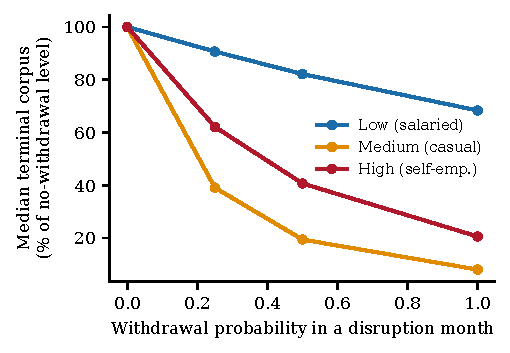
\includegraphics[width=0.9\columnwidth]{figures/fig5_withdrawal.pdf}
\caption{Median terminal corpus under LC75 as a percentage of its no-withdrawal level versus the probability of a withdrawal in a disruption month.}
\label{fig:wd}
\end{figure}

\subsection{R5: The allocation is set by the equity premium (E5)}
\begin{figure*}[!t]
\centering
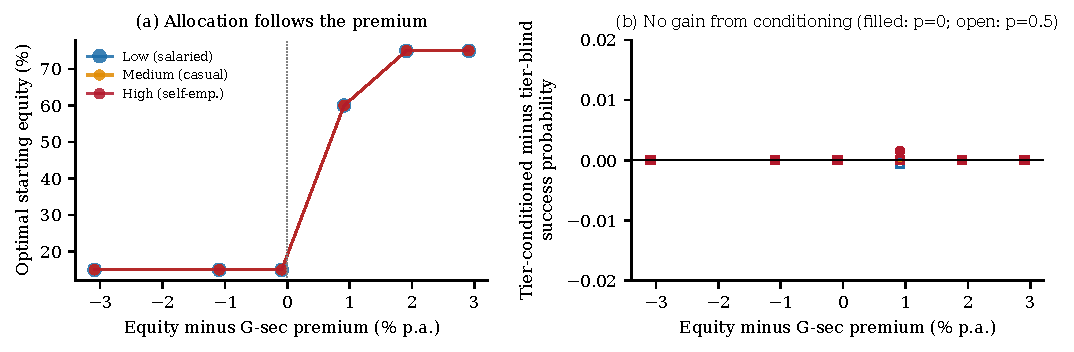
\includegraphics[width=0.95\textwidth]{figures/fig6_premium.pdf}
\caption{(a) Optimal starting equity versus equity premium over G-secs, by tier (curves coincide). (b) Out-of-sample success gain of tier-conditioned over tier-blind allocation (filled: no withdrawals; open: withdrawal probability 0.5).}
\label{fig:prem}
\end{figure*}

Subtracting a constant annual haircut from every bootstrapped equity month (preserving volatility, correlation and regime structure) shows that the optimal allocation tracks the equity-minus-G-sec premium (Fig.~\ref{fig:prem}a, Table~\ref{tab:prem}). The optimum is $75\%$ starting equity at premiums of $+2.9\%$ and $+1.9\%$, $60\%$ at $+0.9\%$, and $15\%$ at $-0.1\%$ and below: the switch from maximum to minimum equity occurs at a premium of roughly $0$--$1\%$ per year, and does so \emph{identically in every tier}. The paired success gain of tier-conditioning over the tier-blind policy never exceeds $0.0015$ (and $0.0005$ with $p=0.5$ withdrawals; Fig.~\ref{fig:prem}b).

\begin{table}[!htbp]
\centering
\caption{Equity-premium break-even (success-maximizing starting equity)}
\label{tab:prem}
\small
\begin{tabular}{cccc}
\hline
Premium & Optimal start & Max $|$gain$|$ & Max $|$gain$|$ \\
(\% p.a.) & equity, all tiers & $p=0$ & $p=0.5$ \\
\hline
+2.91 & 75\% & 0 & 0 \\
+1.91 & 75\% & 0 & 0 \\
+0.91 & 60\% (75\% for some tiers, $p{=}0.5$) & .0015 & .0005 \\
$-$0.09 & 15\% & 0 & 0 \\
$-$1.09 & 15\% & 0 & 0 \\
$-$3.09 & 15\% & 0 & 0 \\
\hline
\end{tabular}
\end{table}

\subsection{R6: The result is robust to the income assumptions (E5)}
We regenerated the synthetic population under nine scenarios---baseline; informal disruption rate $\times2$ and $\times0.5$; informal contribution propensity $\times0.5$ and $\times1.5$; PLFS dispersion $\times1.5$ and $\times0.67$; subsistence floor Rs~3{,}000 and Rs~8{,}000---at two premium settings (none and $2\%$ haircut) for the three tiers, giving 54 cells. In each cell we compare the tier-conditioned and tier-blind success-maximizing policies on common market paths and compute a 95\% paired bootstrap confidence interval (2{,}000 resamples over market trials). No interval excludes zero in any of the 54 cells; the largest absolute gain is $0.004$ (Fig.~\ref{fig:forest}, Table~\ref{tab:robust}). In 43 of the 54 cells the two policies are identical; in the remaining 11 the differences are within sampling noise.

\begin{figure}[!htbp]
\centering
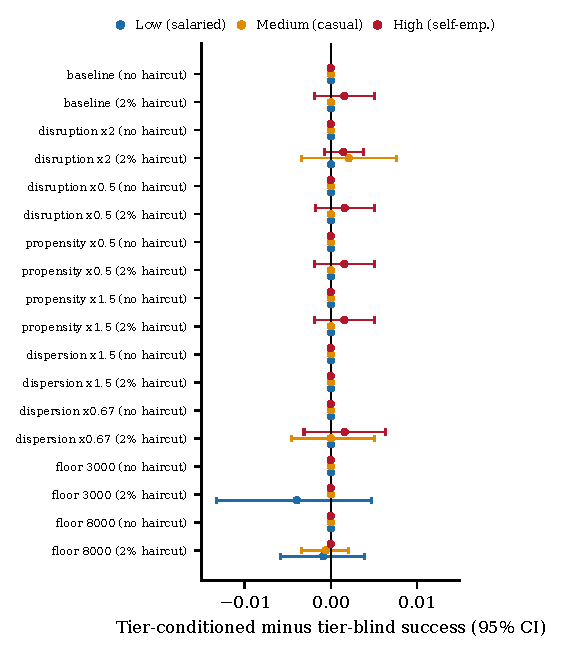
\includegraphics[width=0.8\columnwidth]{figures/fig7_robustness.pdf}
\caption{Paired success gain of tier-conditioned over tier-blind allocation with 95\% bootstrap confidence intervals for 9 scenarios $\times$ 2 premium settings $\times$ 3 tiers.}
\label{fig:forest}
\end{figure}

\begin{table}[!htbp]
\centering
\caption{Robustness by scenario (6 cells each: 2 premium settings $\times$ 3 tiers)}
\label{tab:robust}
\small
\begin{tabular}{lccc}
\hline
Scenario & Identical & Max $|$gain$|$ & Widest 95\% CI \\
 & policies & & width \\
\hline
Baseline & 5/6 & .0015 & .0070 \\
Disruption $\times2$ & 4/6 & .0021 & .0109 \\
Disruption $\times0.5$ & 5/6 & .0016 & .0068 \\
Propensity $\times0.5$ & 5/6 & .0015 & .0070 \\
Propensity $\times1.5$ & 5/6 & .0015 & .0070 \\
Dispersion $\times1.5$ & 6/6 & 0 & 0 \\
Dispersion $\times0.67$ & 4/6 & .0016 & .0096 \\
Floor Rs 3,000 & 5/6 & .0040 & .0180 \\
Floor Rs 8,000 & 4/6 & .0009 & .0098 \\
\hline
\end{tabular}
\end{table}

%--------------------------------------------------------------------------
\FloatBarrier
\section{Discussion}
\textbf{Why does allocation decouple from volatility?} A glide path acts on \emph{returns}; income volatility acts on \emph{contributions}. Over a window with a $+2.9\%$ equity premium, extra equity raises every cohort's chance of reaching its target, and the shortfall measure, being a ratio to cumulative contributions, is dominated by market returns. Withdrawals scale outcomes down but, because the optimum is determined by ranking candidate allocations, do not reorder them. The break-even analysis makes this explicit: the same premium that moves the optimum for one tier moves it identically for all.

\textbf{Implications.} The evidence indicates that informal workers' retirement outcomes are shaped mainly by contribution regularity and access to liquidity, not by the fine tuning of the equity schedule: reforms that raise contribution continuity (automatic debit, matched or smoothed contributions) or that provide liquidity without forced asset sales would address the dominant source of difference. For the glide path itself, the risk-budget interface (next section) allows a subscriber to choose a tolerance for intra-horizon shortfall, which maps transparently to an allocation.

\textbf{What would change the conclusion.} H1 is not refuted in general, only in the policy classes and objectives we tested. Plausible extensions include (i) contribution-aware, state-dependent rules that respond to realized contribution history rather than age alone; (ii) targets that scale with a cohort's income (replacement-rate goals); (iii) behavioral responses such as selling after losses; and (iv) return regimes containing deep, prolonged drawdowns, which the 2009--2026 window lacks.

%--------------------------------------------------------------------------
\FloatBarrier
\section{Risk-Budget Recommender}
To make the analysis usable we expose the engine through a function and a thin REST endpoint (\texttt{POST /recommend}). Inputs are a volatility tier or employment type and a risk budget $\varepsilon$; the response contains the selected glide path by age, terminal-corpus percentiles (P10--P90) for the recommended path, LC50 and LC75, the probability of reaching the LC50-median target, shortfall probabilities, and the cohort's contribution-skip rate. Because $\varepsilon$ is enforced on the search seed, the response also reports whether the budget is met on fresh market draws. For example, for a self-employed subscriber with $\varepsilon=0.05$ the recommended path (55\% starting equity) has a median corpus of Rs~6.6M against Rs~6.0M for LC50 and a shortfall probability of $0.060$ out of sample, which the service flags as marginally above budget. Projections are in nominal rupees for ages 25--60 under the historical premium and are not financial advice.

%--------------------------------------------------------------------------
\FloatBarrier
\section{Limitations and Future Work}
\emph{Synthetic population.} Calibration uses PLFS aggregates at cell level; the individual-dispersion multipliers, persistence, growth, disruption rates, propensities, subsistence floor and withdrawal rule are labelled assumptions (Table~\ref{tab:assump}); we perturbed the main ones but cannot validate against subscriber microdata. \emph{Single return source and window.} Bootstrap uses SBI Tier~I returns (207 months) in a strong-equity regime; the premium sweep addresses the level of the premium but not additional regimes. \emph{Policy class and objectives.} Candidates are three-parameter glide paths with a fixed corporate/G-sec split on a coarse grid (about 100 candidates in the frontier analysis, 20 in the stress and robustness runs); targets are relative to each scenario's LC50 median and values are nominal; no decumulation phase is modelled. \emph{Statistics.} Confidence intervals resample market trials; selection is in-sample on one seed and validation on another.

Future work includes contribution-aware policies, income-replacement targets, regime-rich or multi-fund return sources (e.g.\ additional pension fund managers), unit-level PLFS microdata, richer withdrawal and behavioral models, and a client-facing dashboard for the recommender.

%--------------------------------------------------------------------------
\FloatBarrier
\section{Conclusion}
We asked whether conditioning the NPS glide path on income volatility can better serve informal workers. Using a reproducible simulation combining real NAV data with a PLFS-calibrated synthetic population, we found that volatility profoundly reduces and disperses accumulation but leaves the optimal allocation unchanged: under terminal, path-dependent, combined, liquidity and risk-budget formulations, and across 54 robustness cells, tier-conditioned allocations are indistinguishable from tier-blind ones, while the optimal equity share is governed by the equity premium over G-secs and flips between roughly $0$ and $1\%$ per year. The policy implication is to prioritize contribution regularity and liquidity design, with risk-budget-based allocation as a transparent way to choose among glide paths. All code, assumptions and figures are released for replication.

\begin{thebibliography}{00}
\bibitem{pfrda} Pension Fund Regulatory and Development Authority, \emph{Annual Report 2023--24}, New Delhi, India.
\bibitem{plfs} Ministry of Statistics and Programme Implementation (NSO), \emph{Periodic Labour Force Survey (PLFS), Annual Report 2023--24}, Government of India.
\bibitem{npsnav} NPSNAV, ``NPS NAV data API,'' \url{https://npsnav.in}, accessed 2026.
\bibitem{merton} R.~C. Merton, ``Lifetime portfolio selection under uncertainty: The continuous-time case,'' \emph{Rev. Econ. Stat.}, vol.~51, no.~3, pp. 247--257, 1969.
\bibitem{samuelson} P.~A. Samuelson, ``Lifetime portfolio selection by dynamic stochastic programming,'' \emph{Rev. Econ. Stat.}, vol.~51, no.~3, pp. 239--246, 1969.
\bibitem{bms} Z.~Bodie, R.~C. Merton, and W.~F. Samuelson, ``Labor supply flexibility and portfolio choice in a life cycle model,'' \emph{J. Econ. Dyn. Control}, vol.~16, no.~3--4, pp. 427--449, 1992.
\bibitem{viceira} L.~M. Viceira, ``Optimal portfolio choice for long-horizon investors with nontradable labor income,'' \emph{J. Finance}, vol.~56, no.~2, pp. 433--470, 2001.
\bibitem{cgm} F.~F. Cocco, F.~J. Gomes, and P.~J. Maenhout, ``Consumption and portfolio choice over the life cycle,'' \emph{Rev. Financial Stud.}, vol.~18, no.~2, pp. 491--533, 2005.
\bibitem{gm} F.~Gomes and A.~Michaelides, ``Optimal life-cycle asset allocation: Understanding the empirical evidence,'' \emph{J. Finance}, vol.~60, no.~2, pp. 869--904, 2005.
\bibitem{cv} J.~Y. Campbell and L.~M. Viceira, \emph{Strategic Asset Allocation: Portfolio Choice for Long-Term Investors}. Oxford, U.K.: Oxford Univ. Press, 2002.
\bibitem{bengen} W.~P. Bengen, ``Determining withdrawal rates using historical data,'' \emph{J. Financial Planning}, vol.~7, no.~4, pp. 171--180, 1994.
\bibitem{efron} B.~Efron, ``Bootstrap methods: Another look at the jackknife,'' \emph{Ann. Statist.}, vol.~7, no.~1, pp. 1--26, 1979.
\bibitem{kunsch} H.~R. K\"unsch, ``The jackknife and the bootstrap for general stationary observations,'' \emph{Ann. Statist.}, vol.~17, no.~3, pp. 1217--1241, 1989.
\bibitem{politis} D.~N. Politis and J.~P. Romano, ``The stationary bootstrap,'' \emph{J. Amer. Statist. Assoc.}, vol.~89, no.~428, pp. 1303--1313, 1994.
\end{thebibliography}

\end{document}
